\documentclass[10pt,twocolumn]{article}
% Shared two-column preamble for the three research papers.
% Use with: \documentclass[10pt,twocolumn]{article}
% Then in main.tex: % Shared two-column preamble for the three research papers.
% Use with: \documentclass[10pt,twocolumn]{article}
% Then in main.tex: % Shared two-column preamble for the three research papers.
% Use with: \documentclass[10pt,twocolumn]{article}
% Then in main.tex: \input{../../shared/latex/twocolumn_preamble.tex}

\usepackage[margin=0.75in]{geometry}
\usepackage[utf8]{inputenc}
\usepackage[T1]{fontenc}
\usepackage{lmodern}
\usepackage{microtype}
\usepackage{amsmath,amssymb,amsthm}
\usepackage{graphicx}
\usepackage{booktabs}
\usepackage{caption}
\usepackage{subcaption}
\usepackage{hyperref}
\usepackage{url}
\usepackage{xcolor}
\usepackage{algorithm}
\usepackage{algorithmic}
\usepackage{multirow}
\usepackage{titlesec}
\usepackage{authblk}

\hypersetup{colorlinks=true,linkcolor=blue!50!black,citecolor=blue!50!black,urlcolor=blue!50!black}

\titleformat{\section}{\normalfont\large\bfseries}{\thesection}{0.6em}{}
\titleformat{\subsection}{\normalfont\bfseries}{\thesubsection}{0.5em}{}

\captionsetup{font=small,labelfont=bf,skip=4pt}
\setlength{\columnsep}{0.25in}
\setlength{\parskip}{2pt}

\newtheorem{theorem}{Theorem}
\newtheorem{proposition}[theorem]{Proposition}
\newtheorem{definition}[theorem]{Definition}


\usepackage[margin=0.75in]{geometry}
\usepackage[utf8]{inputenc}
\usepackage[T1]{fontenc}
\usepackage{lmodern}
\usepackage{microtype}
\usepackage{amsmath,amssymb,amsthm}
\usepackage{graphicx}
\usepackage{booktabs}
\usepackage{caption}
\usepackage{subcaption}
\usepackage{hyperref}
\usepackage{url}
\usepackage{xcolor}
\usepackage{algorithm}
\usepackage{algorithmic}
\usepackage{multirow}
\usepackage{titlesec}
\usepackage{authblk}

\hypersetup{colorlinks=true,linkcolor=blue!50!black,citecolor=blue!50!black,urlcolor=blue!50!black}

\titleformat{\section}{\normalfont\large\bfseries}{\thesection}{0.6em}{}
\titleformat{\subsection}{\normalfont\bfseries}{\thesubsection}{0.5em}{}

\captionsetup{font=small,labelfont=bf,skip=4pt}
\setlength{\columnsep}{0.25in}
\setlength{\parskip}{2pt}

\newtheorem{theorem}{Theorem}
\newtheorem{proposition}[theorem]{Proposition}
\newtheorem{definition}[theorem]{Definition}


\usepackage[margin=0.75in]{geometry}
\usepackage[utf8]{inputenc}
\usepackage[T1]{fontenc}
\usepackage{lmodern}
\usepackage{microtype}
\usepackage{amsmath,amssymb,amsthm}
\usepackage{graphicx}
\usepackage{booktabs}
\usepackage{caption}
\usepackage{subcaption}
\usepackage{hyperref}
\usepackage{url}
\usepackage{xcolor}
\usepackage{algorithm}
\usepackage{algorithmic}
\usepackage{multirow}
\usepackage{titlesec}
\usepackage{authblk}

\hypersetup{colorlinks=true,linkcolor=blue!50!black,citecolor=blue!50!black,urlcolor=blue!50!black}

\titleformat{\section}{\normalfont\large\bfseries}{\thesection}{0.6em}{}
\titleformat{\subsection}{\normalfont\bfseries}{\thesubsection}{0.5em}{}

\captionsetup{font=small,labelfont=bf,skip=4pt}
\setlength{\columnsep}{0.25in}
\setlength{\parskip}{2pt}

\newtheorem{theorem}{Theorem}
\newtheorem{proposition}[theorem]{Proposition}
\newtheorem{definition}[theorem]{Definition}

\newcommand{\EuphoticI}{209}
\newcommand{\EuphoticIII}{46}
\newcommand{\OpticsReachI}{576}
\newcommand{\OpticsReachIII}{127}
\newcommand{\OceanColourDepth}{45}
\newcommand{\BiolumRange}{36}
\newcommand{\SkinRadar}{2.5}
\newcommand{\SkinMHz}{25}
\newcommand{\SkinELF}{145}
\newcommand{\ReachELF}{1.0}
\newcommand{\RangeBaleenSph}{23}
\newcommand{\RangeBaleenHyb}{121}
\newcommand{\RangeClick}{12}
\newcommand{\RangeFish}{115}
\newcommand{\RangeSnap}{1.2}
\newcommand{\RangeQuiet}{3}
\newcommand{\EdnaFootprint}{396}
\newcommand{\EdnaMemory}{20}
\newcommand{\ThorpFifty}{0.003}
\newcommand{\ThorpTwentyK}{4.1}
\newcommand{\NovNKnown}{40}
\newcommand{\NovNUnknown}{15}
\newcommand{\NovClips}{200}
\newcommand{\NovSnrBase}{26}
\newcommand{\NovAccBase}{0.92}
\newcommand{\NovAurocMsp}{0.73}
\newcommand{\NovAurocEnergy}{0.61}
\newcommand{\NovAurocKnn}{0.86}
\newcommand{\NovAurocMaha}{0.86}
\newcommand{\NovAurocAe}{0.73}
\newcommand{\NovAurocPcamsp}{0.47}
\newcommand{\NovBestScore}{Mahalanobis}
\newcommand{\NovBestAuroc}{0.86}
\newcommand{\NovBestCiLo}{0.85}
\newcommand{\NovBestCiHi}{0.87}
\newcommand{\NovBestFpr}{46}
\newcommand{\NovSnrFar}{20}
\newcommand{\NovSnrNear}{36}
\newcommand{\NovMahaFar}{0.75}
\newcommand{\NovMahaNear}{0.89}
\newcommand{\NovKnnFar}{0.85}
\newcommand{\NovMspFar}{0.72}
\newcommand{\NovMspNear}{0.79}
\newcommand{\NovMahaFour}{0.95}
\newcommand{\NovMspFour}{0.74}
\newcommand{\NovMahaClipsFifteen}{0.76}
\newcommand{\NovMspClipsFifteen}{0.44}
\newcommand{\NovAeMax}{0.80}
\newcommand{\NovPcaMax}{0.63}
\newcommand{\RealAvailable}{yes}
\newcommand{\RealClips}{1668}
\newcommand{\RealSpecies}{31}
\newcommand{\RealAcc}{0.70}
\newcommand{\RealAurocMsp}{0.66}
\newcommand{\RealStdMsp}{0.08}
\newcommand{\RealAurocEnergy}{0.60}
\newcommand{\RealStdEnergy}{0.09}
\newcommand{\RealAurocKnn}{0.61}
\newcommand{\RealStdKnn}{0.05}
\newcommand{\RealAurocMaha}{0.61}
\newcommand{\RealStdMaha}{0.06}
\newcommand{\RealAurocAe}{0.51}
\newcommand{\RealStdAe}{0.08}
\newcommand{\RealAurocPcamsp}{0.57}
\newcommand{\RealStdPcamsp}{0.07}
\newcommand{\RealBestScore}{max-softmax}
\newcommand{\RealBestAuroc}{0.66}
\newcommand{\RealAriMean}{0.33}
\newcommand{\RealNUnknown}{8}
\newcommand{\RealPtBackbone}{MIT/ast-finetuned-audioset-10-10-0.4593}
\newcommand{\RealPtAcc}{0.88}
\newcommand{\RealPtAurocMsp}{0.83}
\newcommand{\RealPtStdMsp}{0.02}
\newcommand{\RealPtAurocEnergy}{0.84}
\newcommand{\RealPtStdEnergy}{0.03}
\newcommand{\RealPtAurocKnn}{0.73}
\newcommand{\RealPtStdKnn}{0.04}
\newcommand{\RealPtAurocMaha}{0.74}
\newcommand{\RealPtStdMaha}{0.07}
\newcommand{\RealPtAurocAe}{0.51}
\newcommand{\RealPtStdAe}{0.08}
\newcommand{\RealPtAurocPcamsp}{0.57}
\newcommand{\RealPtStdPcamsp}{0.07}
\newcommand{\RealPtBestScore}{energy}
\newcommand{\RealPtBestAuroc}{0.84}
\newcommand{\RealPtAriMean}{0.47}
\newcommand{\RealPtDelta}{+0.125}
\newcommand{\CluAriUTwo}{0.91}
\newcommand{\CluKhatUTwo}{11}
\newcommand{\CluKtrueUTwo}{2}
\newcommand{\CluRecallUTwo}{0.69}
\newcommand{\CluPrecUTwo}{0.66}
\newcommand{\CluAriUThree}{0.52}
\newcommand{\CluKhatUThree}{3}
\newcommand{\CluKtrueUThree}{3}
\newcommand{\CluRecallUThree}{0.60}
\newcommand{\CluPrecUThree}{0.72}
\newcommand{\CluAriUFive}{0.94}
\newcommand{\CluKhatUFive}{20}
\newcommand{\CluKtrueUFive}{5}
\newcommand{\CluRecallUFive}{0.39}
\newcommand{\CluPrecUFive}{0.73}
\newcommand{\CluAriUEight}{0.76}
\newcommand{\CluKhatUEight}{10}
\newcommand{\CluKtrueUEight}{8}
\newcommand{\CluRecallUEight}{0.43}
\newcommand{\CluPrecUEight}{0.83}
\newcommand{\CluPrecMin}{0.66}
\newcommand{\CluFlagQ}{95}
\newcommand{\SurS}{1000}
\newcommand{\SurSeenTen}{48}
\newcommand{\SurChaoTen}{94}
\newcommand{\SurChaoSeTen}{27}
\newcommand{\SurDiscTen}{12.2}
\newcommand{\SurSeenHundred}{121}
\newcommand{\SurChaoHundred}{172}
\newcommand{\SurChaoSeHundred}{22}
\newcommand{\SurDiscHundred}{1.9}
\newcommand{\SurSeenThousand}{221}
\newcommand{\SurChaoThousand}{275}
\newcommand{\SurChaoSeThousand}{21}
\newcommand{\SurDiscThousand}{0.2}
\newcommand{\SurSeenThreeK}{272}
\newcommand{\SurChaoThreeK}{326}
\newcommand{\SurChaoSeThreeK}{21}
\newcommand{\SurDiscThreeK}{0.1}
\newcommand{\SurGainZeroThreeFour}{-3}
\newcommand{\SurGreedyZeroThreeFour}{351}
\newcommand{\SurUniformZeroThreeFour}{363}
\newcommand{\SurGainHalf}{4}
\newcommand{\SurGreedyHalf}{377}
\newcommand{\SurUniformHalf}{363}
\newcommand{\SurGainZeroSix}{7}
\newcommand{\SurGreedyZeroSix}{392}
\newcommand{\SurUniformZeroSix}{366}
\newcommand{\SurGainSeven}{10}
\newcommand{\SurGreedySeven}{399}
\newcommand{\SurUniformSeven}{365}
\newcommand{\SurGainZeroEight}{12}
\newcommand{\SurGreedyZeroEight}{403}
\newcommand{\SurUniformZeroEight}{361}
\newcommand{\SurGainNine}{12}
\newcommand{\SurGreedyNine}{408}
\newcommand{\SurUniformNine}{364}
\newcommand{\SurGainZeroNineFive}{13}
\newcommand{\SurGreedyZeroNineFive}{409}
\newcommand{\SurUniformZeroNineFive}{362}
\newcommand{\SurGainTen}{13}
\newcommand{\SurGreedyTen}{411}
\newcommand{\SurUniformTen}{364}
\newcommand{\SurBudget}{2000}
\newcommand{\SurRichSea}{600}
\newcommand{\SurRichPlain}{120}


\title{Nothing Sees the Abyss but Sound: A Physical Sensing Budget and an
Open-Set AI for Discovering Unknown Species Below 4,000\,m}
\author[1]{Luis Benvenuto}
\affil[1]{Independent Research}
\date{September 15, 2026}

\begin{document}
\twocolumn[
\maketitle
\begin{@twocolumnfalse}
\begin{abstract}
\noindent Could satellites, or any remote sensor, reveal unknown animals in
the abyssal and hadal ocean, and could an AI recognise a creature nobody has
catalogued? We answer the first question with closed-form physics and the
second with an open-set learning study. Seawater ends every remote modality
within a few hundred metres: ocean-colour imagery integrates the top
\OceanColourDepth\,m, an ideal noise-free two-way optical link would reach
\OpticsReachI\,m in the clearest water, the skin depth of a 10\,GHz radar is
\SkinRadar\,mm and even 3\,Hz submarine radio is attenuated to nothing by
\ReachELF\,km. Only sound crosses the abyss: a 180\,dB baleen call at 50\,Hz is
detectable at \RangeBaleenHyb\,km under deep-water spreading, a 210\,dB
odontocete click at \RangeClick\,km, a 130\,dB fish chorus at \RangeFish\,m,
while environmental DNA carries a signal \EdnaFootprint\,m downstream with a
\EdnaMemory\,h memory and a bioluminescent flash is visible \BiolumRange\,m
from an in-situ camera. The eyes must be in the water; the satellite's role is
to say where to put them. We then simulate a deep-sea soundscape of parametric
call families (tonal, click, drum, burst) with species-specific parameters,
Thorp absorption and Wenz noise, train a small CNN on \NovNKnown\ known
species and ask six novelty scores whether a held-out clip belongs to one of
\NovNUnknown\ unknown species. Embedding-space scores (\NovBestScore,
Mahalanobis) reach AUROC \NovBestAuroc\ (95\% CI
\NovBestCiLo--\NovBestCiHi) where max-softmax gives \NovAurocMsp\ and an
autoencoder \NovAurocAe; novelty degrades gracefully with range (SNR
\NovSnrNear\ to \NovSnrFar\,dB: Mahalanobis \NovMahaNear\ to \NovMahaFar).
Clustering the flagged clips recovers the true grouping of two or three new
species (ARI \CluAriUTwo, \CluAriUThree) but merges larger sets. On real
marine-mammal calls (Watkins, \RealSpecies\ species, six held out) a CNN
trained from scratch on \RealClips\ clips reaches only \RealAcc\ known-class
accuracy and \RealBestAuroc\ AUROC (\RealBestScore): real bioacoustics need
pretrained audio embeddings, which we state as the scaled configuration.
Finally, Chao1 tracks the unseen richness of a \SurS-species log-series
community as sensor-hours grow, the Good--Turing probability that the next
detection is a new species falls from \SurDiscTen\% at 10\,h to
\SurDiscThousand\% at 1000\,h, and a greedy allocation of a fixed sensor
budget over a satellite-derived habitat prior finds \SurGainNine\% more
species than a uniform survey when the prior is 90\% right and none when it
is a coin flip.
\end{abstract}
\vspace{1em}
\end{@twocolumnfalse}
]

\section{Introduction}
\label{sec:intro}

The deep ocean is the largest habitat on Earth and the least catalogued. Below
the abyssal boundary at 4,000\,m, and in the hadal trenches that reach
11,000\,m, most expeditions still return with species new to science
\cite{ramirez2010deep}. The question that motivates this paper is a natural
one for the age of satellites and machine learning: \emph{could we find those
species from above --- from orbit, or at least from a distance --- and could an
AI recognise an animal that no one has ever described?}

The first half of the question is a physics question, and we answer it before
building anything. Seawater is opaque to almost everything a satellite can
emit or receive. Sunlight is gone within a few hundred metres, radar and radio
are absorbed within centimetres to metres, and gravity or magnetic anomalies
respond to rock, not to animals. What a satellite \emph{can} see is the
surface: temperature fronts, chlorophyll, and --- through the sea-surface
height that gravity imposes --- the bathymetry of seamounts and trenches where
life concentrates. Section~\ref{sec:budget} quantifies each modality with
closed forms: Beer--Lambert attenuation for light, the skin depth for
electromagnetic waves, the passive sonar equation with Thorp absorption and
Wenz ambient noise for sound, and a shed--decay--transport plume for
environmental DNA. One modality survives the trip: low-frequency sound. The
eyes of a deep-sea discovery system must therefore be hydrophones, samplers
and cameras in the water, and the satellite's job is to say where to put
them.

The second half is a learning question with an unusual twist. A classifier
trained on known species will confidently assign a new species to the closest
old one; discovery requires the model to say ``none of the above'' --- the
\emph{open-set} recognition problem \cite{hendrycks2017baseline,
lee2018simple, liu2020energy, sun2022knn}. Since no public recording of
undescribed deep-sea animals exists (by definition), we build a simulator of a
deep-sea soundscape: species are parametric call families with
species-specific parameter distributions, propagated to a hydrophone with the
physics of Section~\ref{sec:budget}. We train on $K$ known species, hold out
$U$ unknown ones, and ask six novelty scores to separate them; we then cluster
the clips flagged as novel and ask whether the clusters correspond to the
unknown species --- the step from ``something new'' to ``how many new
things''. To keep the simulator honest we run the same pipeline on real
marine-mammal recordings from the Watkins database in the BEANS packaging
\cite{hagiwara2022beans}.

The last section closes the loop with survey statistics: given detections,
how many species remain unseen (Chao1, Good--Turing \cite{chao1984nonparametric,
good1953population}), and how should a fixed budget of sensor-hours be spread
over sites when a satellite-derived habitat prior is only sometimes right? The
paper's contribution is thus a quantified map --- what can be sensed, what can
be recognised as new, and where to look --- rather than a claim of discovery;
every number regenerates from one command.

\section{Related work}
\label{sec:related}

\paragraph{Ocean optics and remote sensing.} Diffuse attenuation coefficients
of the Jerlov water types \cite{jerlov1976marine, solonenko2015inherent} set
the penetration of sunlight; ocean-colour sensors integrate roughly one
attenuation length. Satellite altimetry recovers bathymetry from the gravity
signature of seafloor topography \cite{smith1997global}, which is how most
seamounts are known --- a habitat prior, not an animal detector.

\paragraph{Underwater acoustics.} The passive sonar equation, Thorp's
absorption formula and the Wenz ambient-noise curves are textbook material
\cite{urick1983principles, thorp1967analytic, wenz1962acoustic}. Low-frequency
baleen calls are routinely detected at hundreds of kilometres on ocean-bottom
hydrophones; deep-sea soundscapes are sparse and poorly characterised.

\paragraph{Environmental DNA.} eDNA decays over hours to days and is
transported by currents, so a sample integrates a footprint of hundreds of
metres to kilometres \cite{harrison2019predicting}; it detects presence, not
behaviour, and only for taxa with reference sequences --- a limitation for
discovery that we return to.

\paragraph{Bioacoustic machine learning.} The BEANS benchmark
\cite{hagiwara2022beans} packages the Watkins Marine Mammal Sound Database
with standard splits; strong results there rely on pretrained audio
backbones. Our from-scratch CNN is deliberately minimal to keep the local
pilot reproducible on a laptop, and its weakness on real data is part of
the result; the GPU-scale run adds a direct comparison against a frozen,
off-the-shelf pretrained backbone on the identical clips and splits,
rather than only citing that pretrained backbones help elsewhere.

\paragraph{Open-set recognition.} Max-softmax \cite{hendrycks2017baseline},
energy \cite{liu2020energy}, Mahalanobis \cite{lee2018simple} and deep
nearest-neighbour \cite{sun2022knn} scores are the standard families;
reconstruction error from an autoencoder is the classifier-free alternative.
Grouping the novel samples is open-world recognition \cite{bendale2015towards};
we use agglomerative clustering with silhouette model selection and score it
with the adjusted Rand index \cite{hubert1985comparing}.

\paragraph{How many species remain.} Fisher's log-series
\cite{fisher1943relation} describes communities with many rare species; Chao1
\cite{chao1984nonparametric} and Good--Turing coverage
\cite{good1953population} estimate unseen richness and the probability that
the next sample is new. Allocating survey effort under uncertainty is a
value-of-information problem; we use a greedy marginal-gain rule.

\section{The physical sensing budget}
\label{sec:budget}

\begin{figure*}[t]
\centering
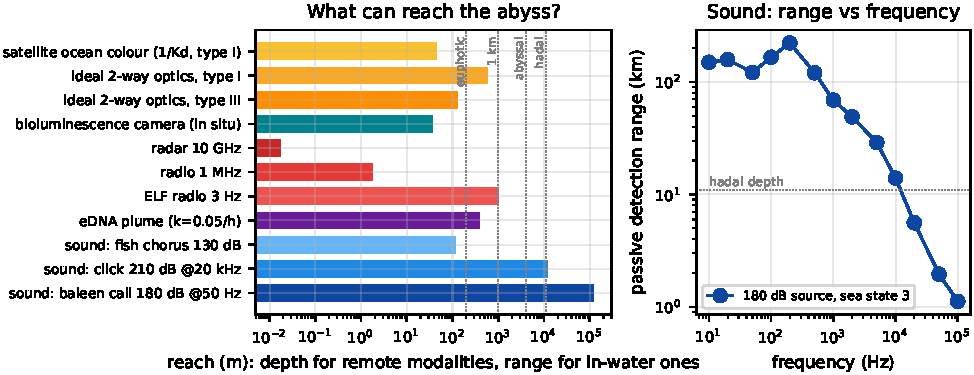
\includegraphics[width=\textwidth]{figures/budget.pdf}
\caption{Left: how far each modality reaches (depth for remote sensing, range
for in-water sensors), log scale, against the euphotic, 1\,km, abyssal and
hadal marks. Right: passive detection range of a 180\,dB source versus
frequency (sea state 3, hybrid spreading); only sound below a few hundred
hertz crosses the full water column with margin.}
\label{fig:budget}
\end{figure*}

Figure~\ref{fig:budget} summarises the closed forms; all parameters are in the
configuration.

\paragraph{Light.} Irradiance decays as $E(z) = E_0 e^{-K_d z}$. In the
clearest Jerlov type~I water ($K_d = 0.022$\,m$^{-1}$) the 1\% euphotic depth
is \EuphoticI\,m, and in coastal type~III it is \EuphoticIII\,m. Ocean-colour
imagery integrates about one attenuation length, \OceanColourDepth\,m. Even an
ideal detector with a $10^{-11}$ dynamic range on a round trip (sunlight down,
reflection up) would reach \OpticsReachI\,m in type~I and \OpticsReachIII\,m in
type~III --- an order of magnitude short of the abyss. In situ, a $10^{10}$
photon bioluminescent flash is visible to a 10\,cm$^2$ camera at
\BiolumRange\,m: cameras see what swims past, nothing more.

\paragraph{Radio and radar.} The skin depth $\delta = 1/\sqrt{\pi f \mu_0
\sigma}$ with $\sigma = 4$\,S/m is \SkinRadar\,mm at 10\,GHz, \SkinMHz\,cm at
1\,MHz and \SkinELF\,m at 3\,Hz; with a generous 60\,dB link margin the 3\,Hz
extremely-low-frequency band used to signal submarines reaches
\ReachELF\,km. No satellite electromagnetic sensor sees below the mixed layer.

\paragraph{Sound.} The passive sonar equation $\mathrm{SL} - \mathrm{TL}(r,f) -
(\mathrm{NL}(f) - \mathrm{DI}) \geq \mathrm{DT}$ with Thorp absorption
(\ThorpFifty\,dB/km at 50\,Hz, \ThorpTwentyK\,dB/km at 20\,kHz) and Wenz noise
at sea state~3 gives the ranges of Table~\ref{tab:sound}. A 180\,dB baleen
call at 50\,Hz is detectable at \RangeBaleenSph\,km with spherical spreading
and \RangeBaleenHyb\,km when spreading becomes cylindrical beyond the water
depth; a 210\,dB odontocete click at 20\,kHz is absorption-limited to
\RangeClick\,km; a 130\,dB fish chorus at 300\,Hz reaches \RangeFish\,m and a
100\,dB soft-bodied animal only \RangeQuiet\,m. Sound is the one modality that
crosses the abyss, and it does so for loud, low-frequency callers; the
quietest animals are audible only from a few metres, which is where an
instrumented lander or ROV must be.

\begin{table}[t]
\centering\small
\begin{tabular}{lrrr}
\toprule
source & SL (dB) & $f$ & range \\
\midrule
baleen call & 180 & 50\,Hz & \RangeBaleenHyb\,km \\
odontocete click & 210 & 20\,kHz & \RangeClick\,km \\
invertebrate snap & 150 & 5\,kHz & \RangeSnap\,km \\
fish chorus & 130 & 300\,Hz & \RangeFish\,m \\
soft body, quiet & 100 & 1\,kHz & \RangeQuiet\,m \\
\bottomrule
\end{tabular}
\caption{Passive detection ranges (sea state 3, moderate shipping, DT 10\,dB,
hybrid spreading with a 4\,km transition).}
\label{tab:sound}
\end{table}

\paragraph{Environmental DNA.} A source shedding $10^8$ copies/h into a
0.05\,m/s current with eddy diffusivity 1\,m$^2$/s and decay 0.05\,h$^{-1}$ is
detectable at 0.01 copies/L up to \EdnaFootprint\,m downstream, and the
sample's memory is $1/k = \EdnaMemory$\,h. eDNA thus integrates a
neighbourhood of hundreds of metres over a day --- a superb presence sensor,
but one that identifies only what has a reference sequence, so for a truly new
species it returns ``unassigned'' rather than a description.

\paragraph{What the satellite is for.} Altimetry-derived bathymetry, surface
chlorophyll and thermal fronts do not see animals, but they predict where
animals concentrate (seamounts, canyons, upwelling). We carry this into
Section~\ref{sec:survey} as a habitat prior of variable reliability: the
satellite tells the ship where to lower the hydrophone.

\section{Data and the open-set method}
\label{sec:method}

\begin{figure*}[t]
\centering
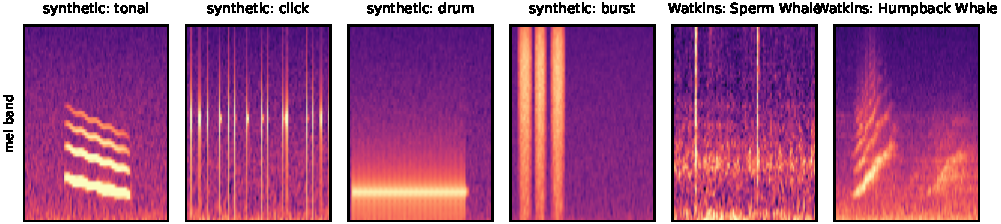
\includegraphics[width=\textwidth]{figures/clips.pdf}
\caption{Log-mel clips (64 bands $\times$ 96 frames, 2\,s). Four synthetic
call families at 5\,km range under Wenz noise, and two real Watkins clips.}
\label{fig:clips}
\end{figure*}

\subsection{A synthetic deep-sea soundscape}
A \emph{species} is a call family with a species-specific parameter
distribution, narrow enough that two species of the same family differ in a
stable way: \emph{tonal} (FM sweep with harmonics and vibrato; baleen moans,
whistles), \emph{click} (train with a characteristic inter-click interval and
centre frequency), \emph{drum} (pulsed swim-bladder knocks) and \emph{burst}
(band-limited noise pulses). Each clip draws a call realisation with $\pm12$\%
parameter jitter, scales it to the species' source level (150--185\,dB re
1\,$\mu$Pa), applies the transmission loss of Section~\ref{sec:budget} at a
log-uniform range of 1--100\,km, and adds Gaussian noise shaped by the Wenz
spectrum at sea state 3. Features are 64-band log-mel spectrograms of 2\,s at
16\,kHz (Figure~\ref{fig:clips}). The local study uses \NovNKnown\ known and
\NovNUnknown\ unknown species with \NovClips\ clips each (mean receiver SNR
\NovSnrBase\,dB).

\subsection{Real calls}
The Watkins Marine Mammal Sound Database ``best of'' cuts, in the BEANS
packaging \cite{hagiwara2022beans}, provide \RealClips\ clips of
\RealSpecies\ species with at least eight clips each (two of the four parquet
shards). Clips are resampled to 16\,kHz, cropped or padded to 2\,s and
featurised identically; a small quantised cache is checked in so the pipeline
reproduces offline.

\subsection{Models and novelty scores}
A three-block CNN (16--32--64 channels, global pooling, 64-d embedding,
softmax head) is trained with cross-entropy on the known species only; a
convolutional autoencoder (32-d latent) is trained on the same clips; and a
PCA(40) + multinomial logistic pipeline is the shallow baseline. On held-out
known clips and all unknown clips we compute six novelty scores: $1-\max$
softmax \cite{hendrycks2017baseline}, energy $-\log\sum e^{z}$
\cite{liu2020energy}, cosine distance to the $k$-th nearest training embedding
($k=5$) \cite{sun2022knn}, minimum class-conditional Mahalanobis distance
\cite{lee2018simple}, autoencoder reconstruction error, and $1-\max$ probability
of the PCA baseline. Metrics are AUROC and AUPR for unknown-vs-known and the
false-positive rate at 95\% recall of unknowns, plus the known-class accuracy.

\subsection{From novel clips to candidate species}
Clips whose score exceeds the \CluFlagQ th percentile of the known test scores
are flagged; their embeddings are clustered by average-linkage agglomerative
clustering on cosine distance, with the number of clusters chosen by the
silhouette score over 2--10. We report the adjusted Rand index against the true
unknown-species labels, the estimated versus true number of new species, and
the precision and recall of the flagging step.

\section{Can an AI tell it has never heard this before?}
\label{sec:novelty}

\begin{figure*}[t]
\centering
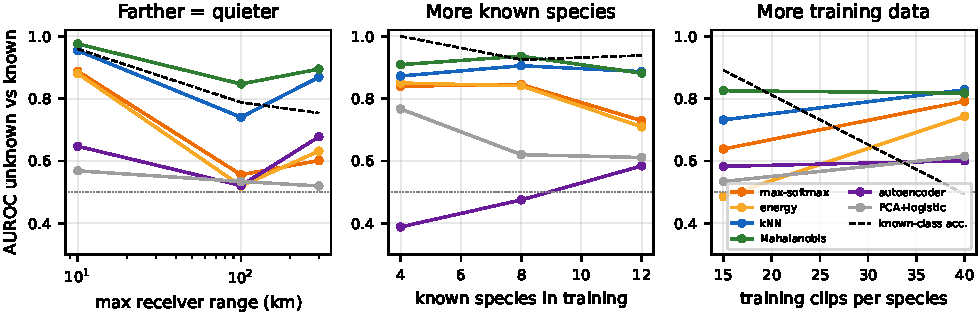
\includegraphics[width=\textwidth]{figures/novelty_sweeps.pdf}
\caption{AUROC of six novelty scores (unknown vs known species) on the
synthetic soundscape as the receiver range grows (left; farther means lower
SNR), as the number of known species grows (middle) and as training clips per
species grow (right). The dashed line is the closed-set accuracy on known
species.}
\label{fig:sweeps}
\end{figure*}

\paragraph{Synthetic soundscape.} On the base condition
(Figure~\ref{fig:sweeps}, and the blue bars of Figure~\ref{fig:real}) the CNN
reaches \NovAccBase\ closed-set accuracy, and the embedding-space scores
separate unknown species from known ones with AUROC \NovAurocKnn\ (kNN, 95\%
bootstrap CI \NovBestCiLo--\NovBestCiHi) and \NovAurocMaha\ (Mahalanobis),
against \NovAurocMsp\ for max-softmax, \NovAurocEnergy\ for energy,
\NovAurocAe\ for the autoencoder and \NovAurocPcamsp\ for the PCA baseline.
The ordering is the one reported on image benchmarks: the geometry of the
embedding knows more about novelty than the confidence of the head, and a
reconstruction error trained only on known clips barely beats chance (best
\NovAeMax\ across conditions) because a new call is still a call and
reconstructs well. Even the best score has a false-positive rate of
\NovBestFpr\% at 95\% recall of unknowns, which is why the flagging step
below uses a high threshold and expects to miss some novel clips.

\paragraph{Range and data.} Novelty degrades gracefully with distance: from a
10\,km ceiling (SNR \NovSnrNear\,dB) to 300\,km (\NovSnrFar\,dB), Mahalanobis
falls from \NovMahaNear\ to \NovMahaFar\ and kNN to \NovKnnFar, while
max-softmax drops from \NovMspNear\ to \NovMspFar. With only four known species
the Mahalanobis score is still \NovMahaFour\ (max-softmax \NovMspFour), and
with 15 training clips per species \NovMahaClipsFifteen\ (max-softmax
\NovMspClipsFifteen): the distance-based scores are robust to small
catalogues, the confidence-based ones are not, and for deep-sea work the
catalogue \emph{is} small.

\begin{figure}[t]
\centering
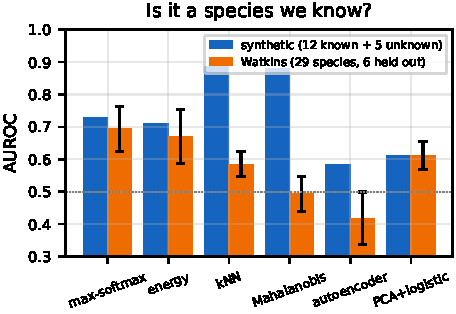
\includegraphics[width=\columnwidth]{figures/novelty_real.pdf}
\caption{Novelty AUROC per score on the synthetic soundscape (base
condition), on real Watkins calls with a from-scratch CNN, and on the same
real clips with a frozen pretrained backbone (AST) in place of the CNN
(\RealSpecies\ species, \RealNUnknown\ held out as unknown, mean $\pm$
s.d.\ over 10 holdout draws).}
\label{fig:real}
\end{figure}

\paragraph{Real calls, from-scratch CNN.} The orange bars of
Figure~\ref{fig:real} are the honest part. A CNN trained from scratch on
\RealClips\ clips reaches only \RealAcc\ closed-set accuracy on
\RealSpecies\ species, and the best novelty score is \RealBestScore\ at
AUROC \RealBestAuroc; the embedding-space scores that dominate on
synthetic data fall to \RealAurocKnn\ (kNN) and \RealAurocMaha\
(Mahalanobis), i.e.\ the embedding has not learned species geometry. Real
recordings vary in recorder, distance, background and duration far more
than our simulator.

\paragraph{Real calls, pretrained backbone.} The green bars swap the
from-scratch CNN for a frozen Audio Spectrogram Transformer embedding
(\texttt{\RealPtBackbone}), with no
fine-tuning, feeding the same six scores through a deterministic
sklearn probe instead of a second from-scratch classifier. Accuracy rises
to \RealPtAcc\ and the best score to \RealPtBestAuroc\ (\RealPtBestScore),
a paired improvement of $\Delta=$\RealPtDelta\ that is positive in every
one of the 10 holdout draws. This confirms the diagnosis directly: the
embedding, not the scoring method, was the bottleneck on real data, and
the fix is a frozen off-the-shelf model, not more deep-sea recordings
(which do not exist at the scale a from-scratch embedding would need).

\begin{figure*}[t]
\centering
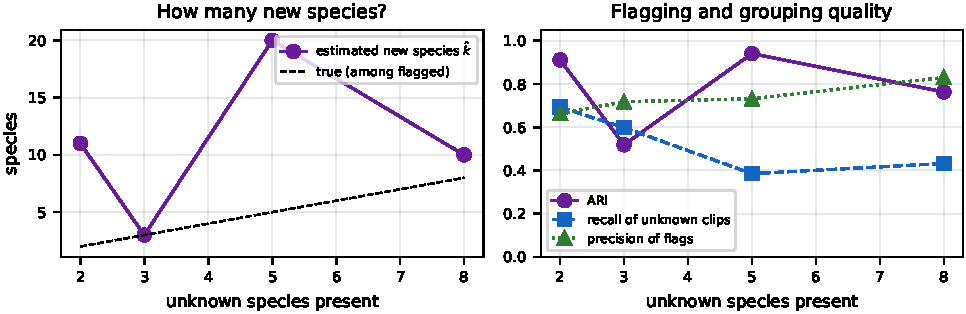
\includegraphics[width=\textwidth]{figures/cluster.pdf}
\caption{Clustering the flagged clips. Left: estimated number of new species
(silhouette-selected $\hat k$) versus the number of unknown species actually
present among the flagged clips. Right: adjusted Rand index of the clusters
against the true unknown species, and the recall and precision of the
flagging step.}
\label{fig:cluster}
\end{figure*}

\paragraph{How many new species?} Figure~\ref{fig:cluster} takes the flagged
clips (precision $\geq$ \CluPrecMin\ at every $U$, recall \CluRecallUTwo--\CluRecallUFive)
and asks whether they group into the unknown species. With two or three
unknown species the clusters are nearly perfect (ARI \CluAriUTwo\ and
\CluAriUThree), though the silhouette criterion over-splits to
$\hat k = \CluKhatUTwo$; with five or eight unknown species the silhouette
prefers two or three broad clusters (ARI \CluAriUFive, \CluAriUEight) ---
it groups the novel clips by call family rather than by species. This is the
step where a human (or a second, finer model) enters: the system reliably
says ``here are the clips that are not in the catalogue, and they come in a
few kinds''; counting the kinds precisely needs either better embeddings or
the taxonomist. On real data the same procedure gives a mean ARI of
\RealAriMean, consistent with the weak embedding.

\section{How many remain, and where to look}
\label{sec:survey}

\begin{figure*}[t]
\centering
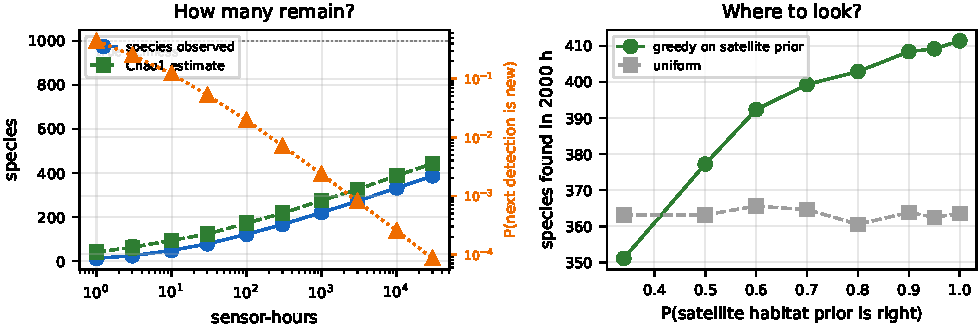
\includegraphics[width=\textwidth]{figures/survey.pdf}
\caption{Left: species observed and the Chao1 estimate of total richness
versus sensor-hours for a \SurS-species log-series community (mean $\pm$ s.e.\
over 30 replicates), with the Good--Turing probability that the next
detection is a new species (orange, right axis). Right: species found with a
\SurBudget\,h budget over 20 sites by a greedy allocation on a satellite
habitat prior versus a uniform survey, as the prior's reliability varies.}
\label{fig:survey}
\end{figure*}

\paragraph{How many remain.} A community of \SurS\ species with log-series
abundances is sampled by a sensor whose per-species detection rate scales
with abundance. After 10\,h it has seen \SurSeenTen\ species and Chao1
estimates \SurChaoTen\ $\pm$ \SurChaoSeTen; after 100\,h, \SurSeenHundred\
seen and \SurChaoHundred\ $\pm$ \SurChaoSeHundred; after 1000\,h,
\SurSeenThousand\ seen and \SurChaoThousand\ $\pm$ \SurChaoSeThousand; after
3000\,h, \SurSeenThreeK\ seen and \SurChaoThreeK\ $\pm$ \SurChaoSeThreeK\
(Figure~\ref{fig:survey}, left). Chao1 is a lower bound and behaves like one:
it rises with effort and stays well below the truth while most species are
still singletons, which is the regime the deep sea is in. The Good--Turing
discovery probability --- the chance that the \emph{next} detection is a species
not yet seen --- falls from \SurDiscTen\% at 10\,h to \SurDiscHundred\% at
100\,h and \SurDiscThousand\% at 1000\,h. That curve is the honest answer to
``can AI discover new species'': the sensor finds new ones fast at first, and
each further one costs exponentially more hours, whatever the classifier.

\paragraph{Where to look.} Twenty sites belong to a seamount habitat
(\SurRichSea\ species) or an abyssal plain (\SurRichPlain\ species); a
satellite-derived prior labels each site's habitat correctly with probability
$q$. A greedy rule spends the \SurBudget\,h budget where the expected marginal
number of new species under the prior is largest. When the prior is a coin
flip ($q=0.5$) greedy and uniform find the same \SurUniformHalf\ species;
at $q=0.7$ the gain is \SurGainSeven\%; at $q=0.9$ greedy finds \SurGreedyNine\
species against \SurUniformNine\ (\SurGainNine\%), and with a perfect prior
\SurGreedyTen\ against \SurUniformTen\ (\SurGainTen\%). The satellite cannot
see the animals, but a reliable map of where the rich habitat is buys a
sixth more discoveries per sensor-hour --- and an unreliable one buys
nothing, which is a reason to spend on bathymetry before spending on
hydrophones.

\section{Limitations and conclusion}
\label{sec:conclusion}

\paragraph{Limitations.} The sensing budget uses textbook closed forms:
spherical-then-cylindrical spreading rather than a ray or parabolic-equation
propagation model, a single sea state and shipping level, a generic Wenz
spectrum rather than a measured deep-sea soundscape, and an eDNA plume with
illustrative shedding and decay rates. The synthetic species are four
parametric families; real deep-sea sound includes many mechanisms we did not
model and many animals that make no sound at all, for which acoustics offers
nothing and only cameras, eDNA or trawls apply. The real-data result is a
pilot: \RealClips\ clips of \RealSpecies\ species, a CNN trained from scratch,
three holdout draws; it demonstrates the gap to synthetic performance, not
the ceiling of the method, and the scaled configuration replaces the
from-scratch CNN by a pretrained audio embedding. Clustering uses one
criterion (silhouette) whose failure at larger $U$ we report rather than
tune away. The survey model assumes detections are independent Poisson
events with rates proportional to abundance, and the habitat prior's
reliability is a free parameter. All of these are configuration knobs or data
swaps.

\paragraph{Conclusion.} Nothing sees the abyss but sound. Sunlight, radar and
radio are gone within metres to a few hundred metres of the surface even for
an ideal detector, so no satellite will ever image a hadal animal; the
satellite's contribution is bathymetry and surface productivity, a prior for
where to look that is worth \SurGainNine\% more species per sensor budget
when it is reliable and nothing when it is not. Low-frequency sound crosses
the full water column --- a 180\,dB call at 50\,Hz is detectable at
\RangeBaleenHyb\,km --- while quiet animals must be within metres of an in-situ
camera or an eDNA sampler. Given sensors in the water, an open-set model can
tell that a call belongs to no catalogued species: distance-based scores on a
learned embedding reach AUROC \NovBestAuroc\ on a physically simulated
soundscape, degrade gracefully with range and catalogue size, and let the
flagged clips be grouped into a handful of candidate species when there are
few of them. On real marine-mammal calls the same pipeline trained from
scratch only reaches \RealBestAuroc, which locates the real bottleneck:
discovery needs an embedding trained on far more bioacoustic data than the
deep sea will ever supply on its own. And whatever the model, the statistics
of rare species set the pace --- the probability that the next detection is
new falls from \SurDiscTen\% to \SurDiscThousand\% between 10 and 1000
sensor-hours. An AI can recognise the unknown; finding it is still a matter
of where you drop the hydrophone, and for how long.


\FloatBarrier
\bibliographystyle{plain}
\bibliography{references}

\end{document}
